% -------------------------------
% CIDaeN: Plantilla para la elaboración del TFM. Versión 0.0 
%
% Luis de la Ossa. UCLM
% 
% Compilar con XeLaTeX 
% -------------------------------
\documentclass[12pt, a4paper]{book}

% -------------------------------
% Información y opciones del documento. Debe editarse.
% -------------------------------
% -------------------------------
% CIDaeN: Plantilla para la elaboración del TFM. Versión 0.0 
%
% Luis de la Ossa. UCLM
% 
% Compilar con XeLaTeX 
% -------------------------------


% -------------------------------
% Comandos comunes
% -------------------------------
\newcommand{\uclm}{Universidad de Castilla-La Mancha\,}
\newcommand{\dsi}{Departamento de Sistemas Informáticos\,}
\newcommand{\esii}{Escuela Superior de Ingeniería Informática de Albacete\,}



% -------------------------------
% Comandos específicos
% -------------------------------
\newcommand{\autor}{Agustín Piqueres Lajarín\,}
\newcommand{\titulo}{Plantilla para la elaboración de la memoria del TFM en el Máster en Ciencia de Datos e Ingeniería de Datos en la Nube (TITULO)\,}
\newcommand{\director}{Daniel González Medina\,}
%\newcommand{\codirector}{Nombre del codirector\,}
\newcommand{\fecha}{Septiembre, 2022\,}






% -------------------------------
% Configuración del documento, paquetes, etc. 
% -------------------------------
% -------------------------------
% CIDaeN: Plantilla para la elaboración del TFM. Versión 0.0 
%
% Luis de la Ossa. UCLM
% 
% Compilar con XeLaTeX 
% -------------------------------


% -------------------------------
% Idioma
% -------------------------------
\usepackage{polyglossia}
\setmainlanguage{spanish}
\PassOptionsToPackage{spanish}{babel}
\usepackage{babel}

% -------------------------------
% Fuente
% -------------------------------
% Cualquier tamaño de texto: {\fontsize{100pt}{120pt}\selectfont tutexto}
\usepackage{anyfontsize}
% Selección de fuentes.
\usepackage{fontspec}
% Espacio entre líneas
\usepackage{setspace}
% Fuentes especiales
\usepackage{textcomp,marvosym,pifont}


% -------------------------------
% Otros paquetes de uso común
% -------------------------------
% Símbolos matemáticos
\usepackage{amsmath,amsfonts,amssymb}
% Gráficos
\usepackage{graphicx}
% Posición arbitraria de los gráficos
\usepackage[absolute,overlay]{textpos}
% Apéndices
\usepackage{appendix}


% -------------------------------
% Esquema de colores
% -------------------------------
% Paquete para la definición de colores
\usepackage[table]{xcolor}
% Esquema de colores
% -------------------------------
% Plantilla del TFG en la ESIIAB-UCLM. Versión 0.0 (Preliminar)
%
% Luis de la Ossa
% 
% Compilar con XeLaTeX 
% -------------------------------


% -------------------------------
% Esquema de colores
% -------------------------------
% Estos balores coinciden con colores de OpenOffice 
% Se pueden redefinir para que coincidan con las paletas de las 
% herramientas utilizadas para hacer las gráficas.
\definecolor{blanco}{RGB}{255,255,255} 
\definecolor{negro}{RGB}{0,0,0}
\definecolor{gris95}{gray}{.95}
\definecolor{gris75}{gray}{.75}
\definecolor{gris50}{gray}{.50}
\definecolor{gris25}{gray}{.25}
\definecolor{rojo}{RGB}{172,39,0}        
\definecolor{azul}{RGB}{2,87,108}        
\definecolor{verde}{RGB}{0,116,70}     
\definecolor{naranja}{RGB}{224, 119, 20} 
\definecolor{mostaza}{RGB}{226, 182, 21} 

% Negrita con color definido 
\newcommand{\bfa}[1]{\textcolor{azul}{\bf #1}} 
\newcommand{\bfr}[1]{\textcolor{rojo}{\bf #1}}
\newcommand{\bfn}[1]{\textcolor{naranja}{\bf #1}}
\newcommand{\bfv}[1]{\textcolor{verde}{\bf #1}}  
\newcommand{\bfm}[1]{\textcolor{mostaza}{\bf #1}} 



% -------------------------------
% Color del tema
% -------------------------------

% Color para los títulos, etc.
%\definecolor{tema}{RGB}{0,0,0}        % Negro 
\definecolor{tema}{RGB}{2,87,108}      % Azul del esquema  

% Negritas con el color del tema
\newcommand{\bft}[1]{\textcolor{tema}{\bf #1}} 



% -------------------------------
% Márgenes
% -------------------------------
% Márgenes de las páginas
\usepackage[
  inner	 =	3cm,   % Margen interior
  outer	 =	2.5cm, % Margen exterior
  top	 =	2.5cm, % Margen superior
  bottom =	2.5cm, % Margen inferior
  includeheadfoot, % Incluye cabecera y pie de página en los márgenes
]{geometry}
% Muestra una regla para comprobar el formato de las páginas (descomentar)
%\usepackage[type=upperleft,showframe,marklength=8mm]{fgruler} 


% -------------------------------
% Renombra tablas y bibliografía
% -------------------------------
\addto\captionsspanish{
	\renewcommand{\listtablename}{Índice de tablas} 
	\renewcommand{\tablename}{Tabla}
	\renewcommand{\bibname}{Referencia bibliográfica}
}


% -------------------------------
% Itemize y enumerate. Control de los espacios.
% -------------------------------
\usepackage{enumitem}
\setitemize{itemsep=0pt}
\setenumerate{itemsep=0pt}
\renewcommand{\labelitemi}{\tiny\bft{$\blacksquare$}}
\renewcommand{\labelitemii}{\bft{$\bullet$}}
\renewcommand{\labelitemiii}{\bft{-}}


% -------------------------------
% Enlaces y colores
% -------------------------------
\usepackage{hyperref}
%\hypersetup{
%    colorlinks,
%    citecolor=black,
%    filecolor=black,
%    linkcolor=black,
%    urlcolor=black
%}

% -------------------------------
% Gestión de elementos flotantes
% -------------------------------
% Para forzar a que las figuras aparezcan antes del fin de una sección.
%\usepackage[section]{placeins}

% Gestión de títulos de los elementos flotantes
\usepackage{caption}
% Subfiguras y títulos en subfiguras
\usepackage{subcaption}

% Títulos
\DeclareCaptionFont{tema}{\color{tema}} % Color
\captionsetup{labelfont={tema, bf}}     % Estilo
\captionsetup{font=normalsize}          % Tamaño
\captionsetup{width=.9\linewidth}       % Anchura del título
 % Distancia de la figura al texto.
\setlength{\intextsep}{1cm} 
\setlength{\textfloatsep}{1cm}         
       

% -------------------------------
% Utilidades para tablas
% -------------------------------
% Para fundir filas en tablas
\usepackage{multirow}
% Para definir columnas con ancho fijo y alineación
\usepackage{array,ragged2e}
\newcolumntype{L}[1]{>{\raggedright\let\newline\\\arraybackslash\hspace{0pt}}m{#1}}
\newcolumntype{C}[1]{>{\centering\let\newline\\\arraybackslash\hspace{0pt}}m{#1}}
\newcolumntype{R}[1]{>{\raggedleft\let\newline\\\arraybackslash\hspace{0pt}}m{#1}}
\usepackage{booktabs}  % Para añadir hrule, toprule... lineas en general

% -------------------------------
% Para tabular
% -------------------------------
\usepackage{tabto}


% -------------------------------
% Formato de títulos, capítulos, etc.
% -------------------------------
\usepackage{titlesec, titletoc}
% Parte
\titleformat{\part}[display]												   	   % Estilo
	{\Huge \centering \color{tema}}                                                % Formato
	{Parte \thepart }                                                              % Etiqueta
	{0.75ex}                                                                       % Separación
	{\bfseries\fontsize{25pt}{40pt}\selectfont}                                    % Entre etiqueta y título            
	[\thispagestyle{empty}]                                                        % Después

% Capítulo		
\titleformat{\chapter}[block]            			 			                    % Estilo  	
	{\vspace{0cm} \flushright \bfseries \LARGE \color{tema}}  	        			% Formato 
	{\thechapter.}                  			  									% Etiqueta
	{0.75ex}                                     									% Separación
	{}                                           									% Entre etiqueta y título
	[\vspace{0.1cm} \rule{0.5\textwidth}{1pt}\vspace*{1cm}\thispagestyle{plain}]    % Después      
  
% Sección
\titleformat{\section}
	{\vspace{5pt}  \Large \color{tema}}
	{\thesection .}
	{0.75ex}
	{}

% Subsección
\titleformat{\subsection}
	{\large \color{tema}}
	{\thesubsection .}
	{0.75ex}
	{}
 
% Subsubsección
\titleformat{\subsubsection}
	{\bf\color{tema}}
	{}
	{0.75ex}
	{}
	 
% Parte (TOC)
\titlecontents{part}[2pc]
  	{\vspace{20pt}\bfseries\filright\Large\color{tema}}
  	{\contentslabel{1.5pc}}{\hspace*{-1.5pc}}
  	{\vspace{5pt}}
  	{}
  
% Capítulo (TOC)
\titlecontents{chapter}[2pc]
  	{\vspace{10pt}\bfseries\large\filright}
  	{\contentslabel{1.5pc}}{\hspace*{-1.5pc}}
  	{\mdseries\titlerule*[0.5pc]{.}\bfseries\contentspage}

% Sección (TOC)
\titlecontents{section}[4pc]
  	{\vspace{5pt}\filright}
  	{\contentslabel{2pc}}{\hspace*{2pc}}
  	{\titlerule*[0.5pc]{.}\contentspage}
  	{\vspace{5pt}

% Subsección (TOC)
\titlecontents{subsection}[6pc]
  	{\vspace{2.5pt}\filright\small\em}
  	{\contentslabel{3pc}}{\hspace*{-3pc}}
  	{\titlerule*[0.5pc]{.}\contentspage} 
  	
  	
% -------------------------------
% Cabeceras y pie de página
% -------------------------------
\usepackage{fancyhdr}
\pagestyle{fancy}
\fancyhf{}

% Permite incluir la parte. Para ello crea \parttitle
\let\Oldpart\part
\newcommand{\parttitle}{}
\renewcommand{\part}[1]{\Oldpart{#1}\renewcommand{\parttitle}{#1}}

% Cabeceras y pies de página
\fancyhead[LE]{}
\fancyhead[RO]{\slshape \leftmark}
\fancyfoot[LE,RO]{\thepage}
\renewcommand{\footrulewidth}{1pt}
\renewcommand{\headrulewidth}{1pt}
\renewcommand{\chaptermark}[1]{\markboth{#1}{}} % Capítulo (Solo texto)
\renewcommand{\chaptermark}[1]{\markboth{\thechapter. #1}{}} % Capítulo (Número y texto)

% Formato plano para las páginas con títulos (solo incluye el pie de página)
\fancypagestyle{plain}{
\fancyhf{}
\fancyhead{}
\fancyfoot[LE,RO]{\thepage}
\renewcommand{\footrulewidth}{1pt}
\renewcommand{\headrulewidth}{0pt}
}

 
% -------------------------------
% Utilidades
% -------------------------------
% Marcas
\newcommand{\pcite}{\bfr{\large[?]}\,} % Cita pendiente: [?] en rojo y negrita.
\newcommand{\ps}{\bfr{\huge[--}\,} % Pricipio de un bloque en sucio
\newcommand{\fs}{\bfr{\huge--]}\,} % Fin de un bloque en sucio.

% Notas
\usepackage[textsize=tiny,spanish,shadow,textwidth=2cm]{todonotes}

% Para generar textos "random"
\usepackage{lipsum} 
 

% -------------------------------
% Algoritmos y código
% -------------------------------

% Se definen entornos específicos para algoritmos y código que permiten
% gestionar los títulos manera similar en ambos casos, y similar al resto
% de elementos flotantes.
\usepackage{newfloat}
\usepackage{float}
\DeclareFloatingEnvironment[ % Algoritmos
  listname = {Índice de algoritmos},
  name = Algoritmo
]{algorithm}

\DeclareFloatingEnvironment[ % Fragmentos de código
  listname = {Índice de listados de código},
  name = Código
]{code}

% Define un estilo para el encabezado de algoritmos y código.
\DeclareCaptionFormat{algcode}{
% OPCIÓN 1 -> Línea debajo del título
\rule{\dimexpr\textwidth\relax}{0.4pt}\vspace{0cm}
#1#2#3
\vspace{-0.2cm}\rule{\dimexpr\textwidth\relax}{0.4pt} % 
% OPCIÓN 2 -> Sin línea debajo del título
%\rule{\dimexpr\textwidth\relax}{0.4pt}\vspace{0cm}
%#1#2#3
}
\captionsetup[algorithm]{format=algcode, width=\linewidth}
\captionsetup[code]{format=algcode, width=\linewidth}

% Opciones específicas para algoritmos.
\usepackage[noend]{algpseudocode}
% Tamaño de letra y separadores
\makeatletter
\renewcommand{\ALG@beginalgorithmic}{\small\hrule\vskip10pt}
\makeatother
% Variables y funciones
\newcommand{\va}[1]{{\it {#1}}}				
\newcommand{\fu}[1]{{\textsc{#1}}}          
% Palabras clave
\renewcommand{\algorithmicrepeat}{\bft{repetir}}
\renewcommand{\algorithmicuntil}{\bft{hasta}}
\renewcommand{\algorithmicend}{\bft{fin}}
\renewcommand{\algorithmicif}{\bft{si}}
\renewcommand{\algorithmicthen}{\bft{entonces}}
\renewcommand{\algorithmicelse}{\bft{si no}}
\newcommand{\algorithmicelsif}{\algorithmicelse\ \algorithmicif}
\newcommand{\algorithmicendif}{\algorithmicend\ \algorithmicif}
\renewcommand{\algorithmicfor}{\bft{para}}
\renewcommand{\algorithmicforall}{\bft{para cada}}
\renewcommand{\algorithmicwhile}{\bft{mientras}}
\renewcommand{\algorithmicdo}{\bft{hacer}}
\renewcommand{\algorithmicprocedure}{\bft{procedimiento}}
\renewcommand{\algorithmicreturn}{\bft{devolver}}
\renewcommand{\algorithmicfunction}{\bft{función}}
\renewcommand{\algorithmicloop}{\bft{iterar}}

% Opciones específicas para código.
\usepackage{listings}
% Aspecto de los listados de código (ejemplo)
% Los colores se han de cambiar y adaptar a los distintos lenguajes de programación.
\lstset{
    language=Python,
    keywordstyle=\bf\color{tema},  
	breaklines=true,    
	basicstyle={\small\ttfamily},
    tabsize=5,
    frame=t % Es importante no cambiar esta opción (es la línea superior) 
}

% -------------------------------
% Cacacteres pifont de uso común (con color)
% -------------------------------
\newcommand{\vmarkt}{\textcolor{tema}{\ding{52}} }  % Checked (V) Tema
\newcommand{\vmarkr}{\textcolor{rojo}{\ding{52}} }  % Checked (V) Rojo
\newcommand{\vmarka}{\textcolor{azul}{\ding{52}} }  % Checked (V) Azul

\newcommand{\xmarkt}{\textcolor{tema}{\ding{55}} }  % Checked (X) Tema
\newcommand{\xmarkr}{\textcolor{rojo}{\ding{55}} }  % Checked (X) Rojo
\newcommand{\xmarka}{\textcolor{azul}{\ding{55}} }  % Checked (X) Azul

\newcommand{\lmarkt}{\textcolor{tema}{\ding{46}} }  % Lápiz Tema
\newcommand{\lmarkr}{\textcolor{rojo}{\ding{46}} }  % Lápiz Rojo
\newcommand{\lmarka}{\textcolor{azul}{\ding{46}} }  % Lápiz Azul

\newcommand{\hmarkt}{\textcolor{tema}{\ding{43}} }  % Mano Tema
\newcommand{\hmarkr}{\textcolor{rojo}{\ding{43}} }  % Mano Roja 
\newcommand{\hmarka}{\textcolor{azul}{\ding{43}} }  % Mano Azula 

\newcommand{\fmarkt}{\textcolor{tema}{\ding{220}} }  % Flechza Tema
\newcommand{\fmarkr}{\textcolor{rojo}{\ding{220}} }  % Flecha Roja 
\newcommand{\fmarka}{\textcolor{azul}{\ding{220}} }  % Flecha Azul

% Documento
\begin{document}

% -------------------------------
% Portada y título
% -------------------------------
% Fuente  de la portada
\setmainfont[Ligatures={NoRequired,NoCommon,NoContextual}]{Calibri}
% -------------------------------
% CIDaeN: Plantilla para la elaboración del TFM. Versión 0.0 
%
% Luis de la Ossa. UCLM
% 
% Compilar con XeLaTeX 
% -------------------------------
\pagestyle{empty}
\begin{titlepage}\null
\begin{textblock*}{3cm}(3cm,2cm) 
\begin{flushleft}

\includegraphics[height=2cm]{figs/logouclm.png}
\end{flushleft}
\end{textblock*}



\begin{textblock*}{2cm}(14cm,2.2cm)  % Corrige la posición porque la imagen tiene margen
\begin{flushright}

\includegraphics[height=1.6cm]{figs/CIDaeN.png}
\end{flushright}
\end{textblock*}



\begin{textblock*}{\textwidth}(3cm,8.5cm) 
\begin{center}\doublespacing 
{\fontsize{18pt}{4pt}\selectfont \bft{TRABAJO FIN DE MÁSTER}}

\bigskip
{\fontsize{18pt}{4pt}\selectfont Máster en Ciencia de Datos e Ingeniería de Datos en la Nube }


\end{center}
\end{textblock*}


\begin{textblock*}{\textwidth}(3cm,14cm) 
\begin{center}\setstretch{2} 
{\fontsize{22pt}{4pt}\selectfont \bft{\titulo}}
\end{center}
\end{textblock*}


\begin{textblock*}{\textwidth}(3cm,20.5cm) 
\begin{flushleft}\doublespacing
{\fontsize{14pt}{4pt}\selectfont \bft{Autor:} \autor}

{\fontsize{14pt}{4pt}\selectfont \bft{Tutor:} \director}

%{\fontsize{14pt}{4pt}\selectfont \bft{Co-Tutor:} \codirector}
\end{flushleft}
\end{textblock*}


\begin{textblock*}{\linewidth}(3cm,25cm) 
\begin{flushright}
{\fontsize{14pt}{4pt}\selectfont \fecha}
\end{flushright}
\end{textblock*}
\end{titlepage}

% -------------------------------
% Fuente del documento.
% -------------------------------
\setmainfont[Ligatures={NoRequired,NoCommon,NoContextual}]{Calibri}

% -------------------------------
% Preámbulo
% -------------------------------
\frontmatter 
% -------------------------------
% CIDaeN: Plantilla para la elaboración del TFM. Versión 0.0 
%
% Luis de la Ossa. UCLM
% 
% Compilar con XeLaTeX 
% -------------------------------



% -------------------------------
% Dedicatoria
% -------------------------------
%\cleardoublepage
%\clearpage
\thispagestyle{empty}

\vspace*{9cm}  
\begin{flushright} \em 
Aquí va la dedicatoria que cada cual \\ 
quiera escribir. El ancho se controla \\ 
manualmente
\end{flushright}

% -------------------------------
% Declaración de autoría
% -------------------------------

%\cleardoublepage
\clearpage
\thispagestyle{plain}
\setcounter{page}{1} \null
\begin{center}
\Large{\bft{Declaración de autoría}}
\end{center}
\vskip1cm

Yo, \quad \ldots \quad, con DNI \quad \ldots \quad, declaro que soy el único autor del trabajo fin de grado titulado ``\quad \ldots \quad'', que el citado trabajo no infringe las leyes en vigor sobre propiedad intelectual, y que todo el material no original contenido en dicho trabajo está apropiadamente atribuido a sus legítimos autores.

\vspace*{2cm}
\begin{center}
Albacete, a \quad \ldots \quad de \quad \ldots \quad de 20 \ldots

\vskip3cm

Fdo.: \autor
\end{center}


% -------------------------------
% Resumen
% -------------------------------
%\cleardoublepage
\clearpage
\thispagestyle{plain}
\begin{center}
\Large{\bft{Resumen}}
\end{center}
\vskip1cm

El CrossFit como deporte como deporte competitivo ha venido ganando adeptos en los últimos años, y el primer paso de clasificación en una competición consiste en realizar una o varias pruebas (\textit{workouts}) que deben ser grabadas y enviadas a la organización para su revisión.

En este trabajo se desarrolla una aplicación para clasificar movimientos de CrossFit como primer paso hacia una aplicación que permita automatizar la revisión de las pruebas enviadas por los atletas. Para llevar a cabo el mismo se crea un conjunto de \textit{clips} de movimientos, basado en videos realizados por competidores de élite de CrossFit perteneciente a la final de los Crossfit Games 2020. El clasificador utilizado se basa en \textit{MoViNets}, una familia de redes neuronales para videos eficiente tanto en términos de computación como de memoria, y se presenta una aplicación desarrollada en AWS. Todo el código está disponible públicamente, y una pequeña librería utilizada para trabajar con \textit{MoViNets} está disponible en \href{https://pypi.org/project/movinets_helper/}{PyPI}.



% -------------------------------
% Agradecimientos
% -------------------------------
%\cleardoublepage
\clearpage
\thispagestyle{plain}
\begin{center}
\Large{\bft{Agradecimientos}}
\end{center}
\vskip1cm

AGRADECIMIENTOS AQUÍ


% -------------------------------
% Índices y tablas
% -------------------------------
\tableofcontents	% Índice
\listoffigures		% Índice de figuras
\listoftables		% Índice de tablas
%\listofalgorithms   % Índice de algoritmos (comentar si no los hay)
%\listofcodes	    % Índice de códigos (comentar si no los hay)
%\cleardoublepage
\clearpage

% -------------------------------
% Documento
% -------------------------------
\mainmatter
% Estilo de página
\pagestyle{fancy}

% Introducción
\chapter{Introducción}


\section{Motivación}

En el presente trabajo se busca desarrollar un modelo que sea capaz de clasificar distintos movimientos de CrossFit. Dentro del este deporte, el proceso para clasificarse para una competición suele ser uno o varios \textit{workouts}\footnote{Se entiende por \textit{workout} a un conjunto de ejercicios variados con movimientos funcionales ejecutados a alta intensidad, ver \href{https://www.crossfit.com/what-is-crossfit}{aquí}.}, que debe ser grabado y enviado a la organización del evento en cuestión, para posibles revisiones del mismo.

Debido a que este deporte viene ganando popularidad con los años, han ido surgiendo más competiciones, y por lo tanto la necesidad de revisar estos videos de los atletas que se presentan. Esta tarea, la de revisar la correcta ejecución y el conteo de repeticiones de un atleta, conlleva la necesidad de un \textit{juez}, una persona encargada de revisar y contar las repeticiones en los eventos.

En el caso de los clasificatorios para las competiciones, esta tarea quizá podría ser automa-tizada, utilizando para ello una aplicación a la que poder subir videos, y que se encargue de hacer de juez, contando las repeticiones de los distintos movimientos.

\section{Objetivos}

Como punto de partida para solucionar el problema previo, se pretence ofrecer solución a una versión simplificada de este problema, una aplicación que permita clasificar entre distintos movimientos de CrossFit. Para ello, es necesario disponer de un conjunto de videos que representen los distintos ejercicios, un modelo que permita clasificar estos videos, así como una aplicación en la que un usuario pueda subir estos videos y obtener el movimiento del que se trata.

\section{Estructura del proyecto}

El trabajo se divide en las siguientes secciones. En la sección \ref{estado_del_arte} se expone el estado del arte actual, mostrando los modelos disponibles en la actualidad que tratan la clasificación de actividades humanas, la explotación de los mismos en el actual entorno \textit{cloud}, así como una breve revisión de trabajos relacionados.

El desarrollo del proyecto contempla las siguientes secciones: La sección \ref{extracción_recolección} presenta la metodología para la extracción de datos y el análisis del conjunto de datos obtenido. A continuación, la sección \ref{deep_learning} trata el tratamiento de los datos necesario para entrenar el modelo, y los resultados obtenidos en el mismo. Por último, la sección \ref{despliegue} explica la arquitectura elegida para el despliegue de la aplicación y ejemplos de uso.

Finalmente, en la sección \ref{conclusiones} se resumen los resultados obtenidos y se proponen lineas de mejora.
 

% Estado del arte
\chapter{Estado del arte}

\section{Deep Learning}

El campo del reconocimiento de acciones se ha vuelto un área de investigación activa en los últimos años (ver \href{https://paperswithcode.com/task/action-recognition-in-videos}{\textit{Action Recognition}}). Si bien las acciones humanas se pueden reconocer de diferentes formas, como el \textit{optical flow} o en representaciones de esqueletos, en este trabajo nos centramos en la clasificación de videos. La clasificación de vídeos consiste en la obtención de una etiqueta representativa del contenido del vídeo, dados los frames que lo componen (ver referencia \href{Video Classification is the task of producing a label that is relevant to the video given its frames}{\textit{Video Classification}}).

Con la introducción del dataset \textit{Kinetics 400} (ver \cite{Kinetics400}) se plantea el primer punto de referencia para la clasificación de acciones en humanos. Debido al tamaño del conjunto de datos, se hace posible entrenar redes neuronales desde cero y permite probar distintas arquitecturas sobre el mismo que posteriormente se pueden ajustar a tareas más a la medida por medio de \textit{fine-tuning} (ver \cite{I3D}).

En el momento de plantearse este trabajo, aparece \textit{MoViNets}, una familia de modelos eficientes tanto en el uso de memoria como en computación, que permite operar con videos en \textit{streaming}, logrando  \textit{accuracies} más elevados en comparación con otros modelos desarro-llados en la literatura con sus versiones más complejas (ver \cite{MoViNets})\footnote{Actualmente el panorama de modelos entrenados sobre Kinetics 600 ha evolucionado mucho, como puede verse en \href{https://paperswithcode.com/sota/action-classification-on-kinetics-600}{Action Classification on Kinetics-600}, incluso añadiendo componentes de audio y texto (subtítulos): \cite{Merlot}.}, que ofrecen buenos resultados sobre \textit{Kinetics 600}, una mejora sobre \textit{Kinetics 600}: \cite{Kinetics600}.

Esta familia de modelos se compone de dos versiones diferentes, que en el paper original llaman \textit{base} y \textit{stream}, con 5 "niveles" de complejidad (desde a0 hasta a5, donde a0 es una arquitectura simplificada, y a5-base obtiene resultados al nivel de \cite{X3D} (ver Tabla 17 en y Tabla 22 respectivamente en \textit{MoViNets}). La gran novedad que aporta este trabajo es la variante \textit{stream}, que permite tratar videos de gran longitud sin tener que tratarlo por todos los frames por completo antes de devolver una predicción, con lo que se hace posible la inferencia en videos de gran longitud y con dispositivos de menor capacidad (ver \href{https://blog.tensorflow.org/2022/04/video-classification-on-edge-devices.html}{aquí}).

ver \cite{UCF101}


\section{Cloud}

texto

\section{Trabajos relacionados}

Meter referencias a artículos y blogs:

Ejemplo tenis:

https://blog.ml6.eu/sports-video-analysis-in-the-real-world-realtime-tennis-action-recognition-using-movinet-stream-813200aa589f

Medium ejemplo de contar repeticiones:

https://towardsdatascience.com/how-i-created-the-workout-movement-counting-app-using-deep-learning-and-optical-flow-89f9d2e087ac

texto
 

%% Algunos elementos
\chapter{Desarrollo del proyecto}

\section{Extracción y recoleccion de datos}

\subsection{Introducción}

En el siguiente apartado se expone la metodología de obtención de los datos de entrena-miento.

Las distintas versiones de MoViNets están entrenadas sobre \href{https://www.deepmind.com/open-source/kinetics}{Kinetics 600}, por lo que para reentrenar el modelo necesitamos \textit{clips} (videos) que representen los movimientos que se quieren predecir.

Si bien no existe un conjunto de datos similar aplicado específicamente a movimientos de crossfit, muchos atletas suben videos a youtube de realizando distintas pruebas y ejercicios. Partiendo de estos videos, se pueden extraer los distintos \textit{clips} (trozos) que representen los movimientos con los que reentrenar el modelo.

Todos los videos descargados pertenecen a la primera etapa de los \href{https://en.wikipedia.org/wiki/2020_CrossFit_Games}{Crossfit Games de 2020}). Este año fue algo atípico debido a la pandemia: La final de la competición se distinguió en dos etapas, una primera en formato online, y la final a la que solo pudieron acceder 10 atletas en total (5 hombres y 5 mujeres). Los videos correspondientes a la primera etapa están todos subidos a YouTube, dentro de las \href{https://www.youtube.com/c/CrossFitGamesTV/playlists}{listas de CrossFit Games}, donde todos los atletas están grabados de forma individual y con la cámara estática, lo que reduce enormemente el ruido de los datos.


\subsection{Proceso de extracción}

Para seleccionar la muestra de videos, se ha partido de 4 \textit{eventos} \footnote{Los videos corresponden a los siguientes eventos, que se pueden encontrar \href{https://games.crossfit.com/workouts/games/2020}{aquí}: \textit{Friendly Fran}, \textit{Damn Diane}, \textit{Nasty Nancy} y \textit{Awful Annie}.} que en total dan pie a 9 movimientos (ver las etiquetas en el siguiente \href{https://gist.github.com/plaguss/58091caefee6acb39ae51cbc241b3cf9/raw/labels.txt}{\textit{gist}}).

De cada \textit{evento} se han seleccionado 20 videos (10 de hombres y 10 de mujeres), de los cuales se han etiquetado 15 repeticiones de cada movimiento presente. Esto nos deja con una muestra de alrededor de 300 repeticiones por movimiento, 2700 clips.

Para descargar los videos se ha utilizado \href{https://github.com/yt-dlp/yt-dlp}{\texttt{yt-dlp}}, todos con la misma resolución (480 x 854p) en formato mp4. El siguiente script: \href{https://github.com/plaguss/tfm-misc/blob/main/scripts/download.py}{\texttt{download.py}}, se ha utilizado para las descargas de todos los videos.

El etiquetado de los videos se ha hecho con \href{https://supervise.ly/}{\textit{Supervisely}} \footnote{Tras probar otras alternativas como \href{https://labelstud.io/}{\textit{LabelStudio}}, \textit{Supervisely} facilita enormemente seleccionar rangos de frames por medio de atajos del teclado.}.
Una vez se ha etiquetado un video, \textit{Supervisely} genera un \texttt{json} con las anotaciones correspondientes al movimiento y los frames en los que se produce.

Para obtener cada uno de los clips se ha utilizado \href{https://github.com/plaguss/tfm-misc/blob/main/scripts/ffmpeg-split.py}{\texttt{ffmpeg-split.py}} \footnote{Este script pertenece al siguiente \href{https://github.com/c0decracker/video-splitter}{repositorio}.}. Las anotaciones se tranforman a un formato que \texttt{ffmpeg-split.py} pueda utilizar por medio de \href{https://github.com/plaguss/tfm-misc/blob/main/scripts/manifester.py}{\texttt{manifester.py}}.

La figura \ref{data_extraction_process} resume el proceso para la obtención de los datos\footnote{Todos los scripts utilizados para la la extracción de los datos se encuentran \href{https://github.com/plaguss/tfm-misc/tree/main/scripts}{aquí}.}.


\begin{figure}[H]
    \centering
		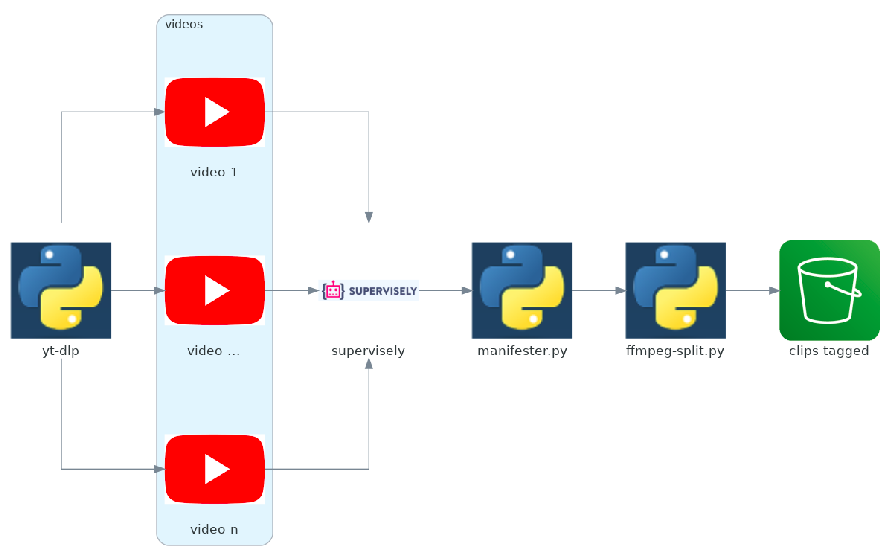
\includegraphics[width=\textwidth]{figs/data_extraction_process_.png}
\caption{Proceso de extración de datos}\label{data_extraction_process}
\end{figure}

\subsection{Datos obtenidos}

Meter tablas resumen de frames y segundos de los vídeos.
\begin{table}[htbp]
\centering
\caption{Estadísticos descriptivos de los frames y duración de los clips}
\label{table_descriptive_stats}
\begin{tabular}{l|lc|lc}
\toprule
{} & \multicolumn{2}{c|}{\textbf{Frames}} & \multicolumn{2}{c}{\textbf{Duración (s)}} \\
{} &    Media & Desviación típica &        Media & Desviación típica \\
\midrule
\textbf{thruster}          &  27.7396 &            4.5060 &       0.9419 &            0.1274 \\
\textbf{chest-to-bar}      &  21.0478 &            7.4233 &       0.7196 &            0.2569 \\
\textbf{double-unders}     &  14.5880 &            1.2740 &       0.4841 &            0.0439 \\
\textbf{ghd}               &  58.9732 &            5.5611 &       1.9654 &            0.1860 \\
\textbf{power clean}       &  67.3567 &           13.0092 &       2.2448 &            0.4337 \\
\textbf{deadlift}          &  24.1229 &            7.1950 &       0.8048 &            0.2395 \\
\textbf{shspu}             &  43.2100 &           15.1247 &       1.4412 &            0.5055 \\
\textbf{ohs}               &  31.9767 &            5.4303 &       1.0664 &            0.1799 \\
\textbf{bar-facing burpee} &  62.0233 &           10.0239 &       2.0688 &            0.3340 \\
\textbf{TOTAL}             &  39.0042 &           7.7275  &       1.3041 &            0.2563 \\
\bottomrule
\end{tabular}
\end{table}



\section{Experimentación con deep learning}

\subsection{Introducción}

En esta sección se explica el modelo seleccionado, el tratamiento aplicado a los datos, el entrenamiento del modelo y los resultados obtenidos.

Existe más de una implementación de los modelos de MoViNets como se puede ver en \href{https://paperswithcode.com/paper/movinets-mobile-video-networks-for-efficient}{\textit{Papers with code}}, pero dado que los autores del \textit{paper} original han desarrollado el mismo utilizando \texttt{tensorflow}, y el repositorio está expuesto de manera pública junto con todos los datos entrenados, se ha decidido utilizar la versión que se puede ver en el \href{repositorio oficial}{https://github.com/tensorflow/models/tree/master/official/projects/movinet} de \textit{MoViNets}.

\subsection{Preprocesado de los datos}

De cara a construir la pipeline para el entrenamiento del modelo, se ha utilizado la API de \href{https://www.tensorflow.org/api_docs/python/tf/data/Dataset}{\texttt{tf.data.Dataset}} ya que permite la ingesta de un conjunto potencialmente grande de datos, así como el procesamiento de los mismos.

La forma más eficiente (BUSCAR REFERENCIA) de leer los videos en el \texttt{Dataset} es escribirlos como \href{https://www.tensorflow.org/api_docs/python/tf/data/TFRecordDataset}{\texttt{tf.data.TFRecordDataset}}, 
\texttt{tf.data.TFRecordDataset}
(REVISAR PARA QUE SALGA LA REFERENCIA)
para lo cuál se deben transformar los videos en formato mp4 a \texttt{tfrecords}. (INSERTAR REFERENCIA A movinets\_helper/writer.py, Y LOS DISTINTOS EJEMPLOS)

Al introducir los videos, se cambia el tamaño para igualarlo al utilizado en el entrenamiento original, 224x224p, y se escalan los valores para que se encuentren en el rango $[0, 1]$.

Para homogeneizar los datos de entrada se ha decidido fijar al número de frames para todos los videos a 10 ($\bar{f}=10$)(BUSCAR REFERENCIA A LOS DATOS UTILIZADOS EN EL PAPER ORIGINAL). Debido a que los vídeos en este conjunto de datos son más cortos que los utilizados en el caso de \textit{Kinetics 600}, se ha seleccionado el número de frames como $\bar{f} = \min_v f_{v}$, donde $f_v$ es el número de frames del vídeo $v$. El menor número de frames corresponde a uno de los vídeos de \textit{double-unders}. Para aquellos vídeos con un número de frames mayor que $\bar{f}$, se seleccionan $\bar{f}$ frames equiespaciados.

En la siguiente imagen podemos ver el ejemplo de uno de los \textit{clips} que entran en la muestra de entrenamiento. Se trata de un \textit{power clean}, donde se pueden ver las distintas imágenes que componen el \textit{clip}.

\begin{figure}[H]
    %\centering
    \centerline{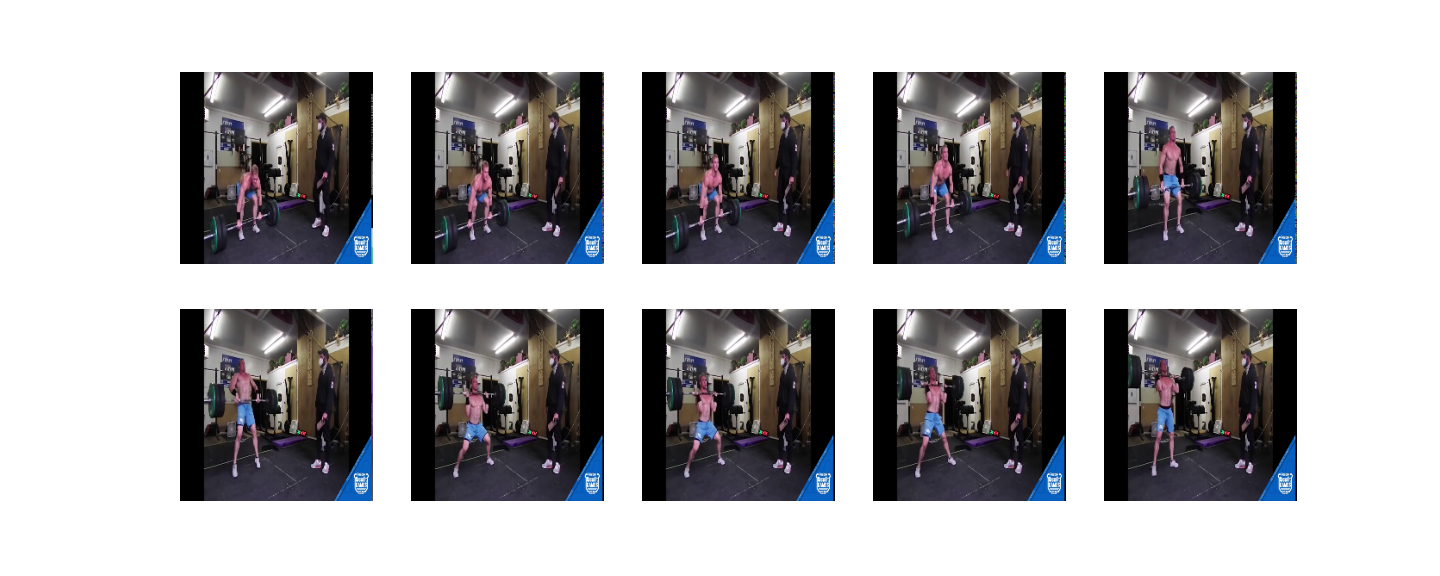
\includegraphics[width=1.25\linewidth]{figs/frames.png}}
\caption{Frames de una muestra de \textit{power clean} de la pipeline de entrenamiento}\label{frames}
\end{figure}

\subsection{Experimentos realizados y resultados}

El modelo se ha entrenado en \href{https://colab.research.google.com/?hl=es}{\textit{Google Colab}} con \textit{Tensorflow 2}. El modelo seleccionado ha sido MoViNets A2 Base\footnote{No ha sido posible hacer fine-tuning del modelo Stream debido a un error en los modelos guardados, ver \href{https://github.com/tensorflow/models/issues/10730}{issue 10730}.}, ya aunque sea necesario utilizar GPU para el fine-tuning, es el modelo más grande (y con mejor capacidad predictiva) que permite hacer inferencia con CPU en un tiempo razonable (BUSCAR REFERENCIA DE LOS AUTORES).

Los hiperparámetros del modelo son los mismos utilizados en el paper original\footnote{Ver apartado \textit{B.1 More Details of the Architectures and Training} de METER BIBLIOGRAFÍA PARA EL PAPER}, con un tamaño de batch igual a 8\footnote{El tamaño del batch seleccionado es el mismo utilizado por los autores en el tutorial a modo de ejemplo sobre el dataset UCF101.}.

La muestra se divide en un $80\%$ (2164 clips) para training, y un $20\%$ (541 clips) para test, donde los ejemplos se distribuyen de manera balanceada (ver figura \ref{sample_sizes}).

\begin{figure}[H]
    \centering
		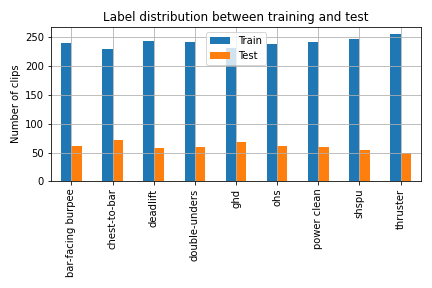
\includegraphics[width=\textwidth]{figs/sample_sizes.png}
\caption{Distribución de las etiquetas entre la muestra de entrenamiento y test}\label{sample_sizes}
\end{figure}

El modelo se ha entrenado por 10 epochs, evaluando top 1 y top 5 accuracy, obteniendo un accuracy de 0.9995 y 1 en entrenamiento y test respectivamente, como podemos observar en la siguiente imagen extraída de \textit{tensorboard.dev}:

\begin{figure}[H]
    \centering
		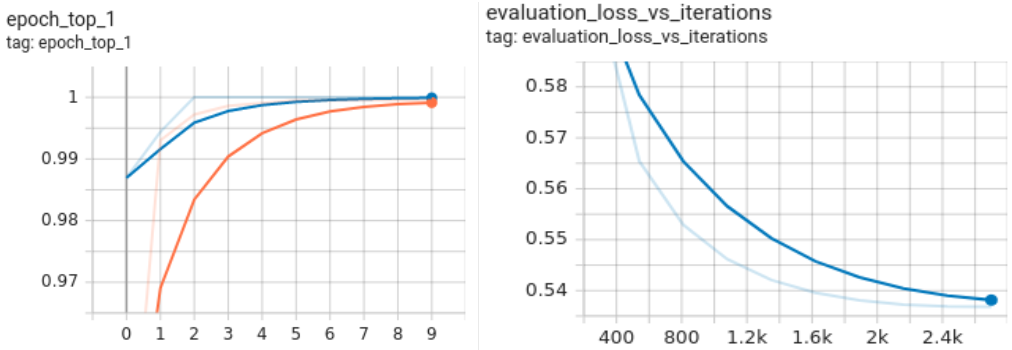
\includegraphics[width=\textwidth]{figs/tensorboard_training.png}
\caption{Top 1 categorial accuracy por epoch y loss frente por número de iteraciones}\label{training}
\end{figure}

El modelo base generaliza a un gran número de movimientos, incluyendo algunos movimientos similares\footnote{Por ejemplo, entre las  \href{https://raw.githubusercontent.com/tensorflow/models/f8af2291cced43fc9f1d9b41ddbf772ae7b0d7d2/official/projects/movinet/files/kinetics_600_labels.txt}{labels de Kinetics 600} se encuentran \textit{squat}, \textit{clean and jerk} o \textit{snatch weight lifting}.} , lo que puede facilitar seguir aprendiendo algunos de movimientos similares.

Por otro lado, los videos en este caso, aunque se han seleccionado de una muestra distinta de atletas, todos ellos son atletas de élite en su deporte, por lo que la ejecución de los movimientos son muy similares entre si, lo que facilita aprender a clasificar los mismos.

Los resultados del entrenamiento se pueden ver en de forma interactiva en el siguiente enlace a \href{https://tensorboard.dev/experiment/UXyupsnMQ2S74vdul3vdbw/#scalars}{\textit{Tensorboard.dev}}.


\subsection{Evaluación de los resultados}

A la hora de evaluar los resultados, empezamos analizando el heatmap de la matriz de confusión. Como se vio al analizar el accuracy en la muestra de test, todos los movimientos se clasifican bien (ver imagen \ref{app_3}).

\begin{figure}[H]
    \centering
		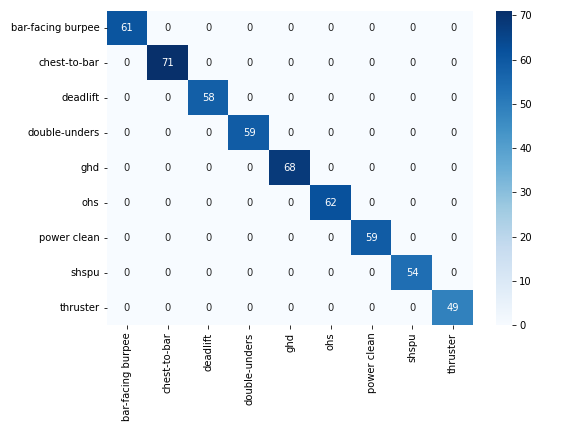
\includegraphics[width=\textwidth]{figs/heatmap_confusion.png}
\caption{Heatmap de la matriz de confusión para la muestra de test.}\label{app_3}
\end{figure}

Con vistas a proporcionar un análisis más robusto en caso de extender el modelo a un mayor número de movimientos o muestras de distintos atletas, puede ser útil la información que proporciona el heatmap de la figura \ref{heatmap_correlations}. La construcción de este gráfico se hace de la siguiente forma:

Partiendo de las probabilidades asignadas a cada vídeo en el período de test, se fija para cada movimiento (cada \textit{label} correcta) y se calculan las correlaciones. Se selecciona la correlación (de Pearson) con el movimiento correctamente etiquetado, y se concatenan todos los vectores columna, de forma que obtenemos una matriz cuadrada. Estas correlaciones ayudan a ver cuáles son los movimientos que más se "confunden" entre si. Dado que las probabilidades deben sumar 1, aquellos movimientos con una correlación negativa más cercana a 1, son aquellos en los que se puede observar una mayor intercambio de probabilidades en la predicción.

\begin{figure}[H]
    \centering
		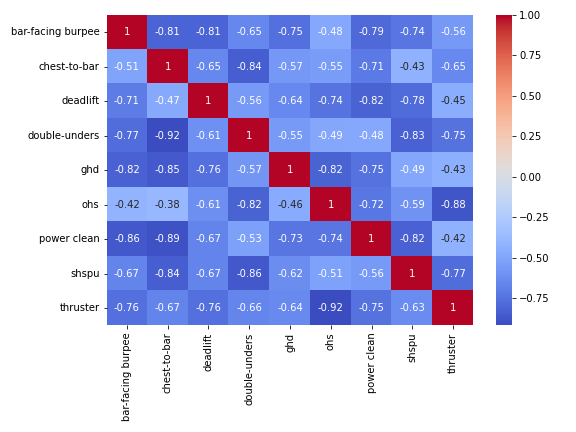
\includegraphics[width=\textwidth]{figs/heatmap_correlations.png}
\caption{Heatmap de correlación entre probabilidades. Para los clips clasificados como $j$, la celda $(i, j)$ representa la correlación entre las probabilidades de predecir el movimiento $i$ y el movimiento $j$.}\label{heatmap_correlations}
\end{figure}

Por ejemplo, si nos fijamos en la columna que corresponde a \textit{ohs}, vemos que el mayor coeficiente de correlación es de $-0.92$, con \textit{thruster}. Esto tiene sentido si se tiene en cuenta que en ambos movimientos, la barra parte de una sentadilla y acaba con la barra bloqueada por encima de la cabeza.

Por último, se puede ver en la siguiente tabla las probabilidades medias y desviación estándar obtenidas para cada movimiento correctamente etiquetado. Esto nos permite ver cuáles son los movimientos que se predicen con una mayor confianza, como en este caso los \textit{double-unders}, o los que menos, los \textit{ohs}. Las probabilidades que dan lugar a esta tabla se pueden ver en \ref{Probabilidades}.


\begin{table}[H]
\centering
\caption{Estadísticos principales }
\label{table_probabilities}
\begin{tabular}{lcc}
\toprule
{} &   Media &  Desviación típica \\
\midrule
double-unders     &  0.8921 &             0.0748 \\
ghd               &  0.8904 &             0.0533 \\
bar-facing burpee &  0.8876 &             0.0756 \\
thruster          &  0.8838 &             0.0590 \\
deadlift          &  0.8746 &             0.0796 \\
shspu             &  0.8731 &             0.0843 \\
chest-to-bar      &  0.8552 &             0.1282 \\
power clean       &  0.8443 &             0.0851 \\
ohs               &  0.8438 &             0.1163 \\
\bottomrule
\end{tabular}
\end{table}


\section{Cloud y despliegue de la aplicación}

En el siguiente apartado se presenta la aplicación para clasificar movimientos de crossfit, la arquitectura elegida así como su funcionamiento para un ejemplo en concreto.

\subsection{Introducción}

Para la explotación del modelo se ha elegido desplegar una aplicación en AWS desarrollada en Plotly Dash. Un usuario solo necesita subir un video en formato mp4, y recibir a cambio las predicciones del mismo. En los siguientes apartados se puede ver la arquitectura de la aplicación en la nube y los resultados obtenidos.

\subsection{Arquitectura cloud}

A continuación se puede ver en la figura \ref{cloud_diagram} el diagrama de la aplicación desplegada en AWS.

El punto de entrada para un usuario es la aplicación desplegada en \href{https://aws.amazon.com/es/ec2/}{\textit{EC2}}, cuyo código se puede ver en el repositorio \href{https://github.com/plaguss/movinets_dash_app}{\texttt{movinets\_dash\_app}}.

La app está desarrollada en \href{https://plotly.com/dash/}{\textit{Dash}}, y ofrece la funcionalidad justa para subir un video en formato mp4 (y mostrarlo), obtener las probabilidades asociadas a cada movimiento, y mostrar ejemplos de los movimientos para los que se ha entrenado el modelo.

Se pueden distinguir dos bloques:
%
\begin{itemize}%
%
\item \textit{App pipeline}.
Por un lado tenemos la aplicación con la que interactúa el usuario.
Se parte de un repositorio público en github que contiene el código del front end. Por medio de \href{https://aws.amazon.com/es/codepipeline/}{AWS CodePipeline} y \href{https://aws.amazon.com/es/codedeploy/}{AWS CodeDeploy} se automatiza el despliegue de la misma en una instancia de \textit{EC2}, que viene desencadenado por medio de un \texttt{git push} a la rama master del repositorio.

\item \textit{Model predictions}.
Al subir un video, este se puede mandar a predecir (solo se reproduce en pantalla por defecto). El proceso en este caso contempla la interacción con el modelo por medio de una función \href{https://aws.amazon.com/es/lambda/}{\textit{AWS Lambda}}. Debido a las restricciones de tamaño de lambda, no es posible desplegar el código de la misma simplemente comprimiendo las dependencias ya que tensorflow por si solo excede el límite. El código de la lambda \href{https://github.com/plaguss/tfm-misc/tree/main/lambda_aws}{(ver aquí)} se debe empaquetar en Docker y subir la imagen a \href{https://aws.amazon.com/es/ecr/}{ECR}. La lambda se encarga por tanto de leer el video, cargar el modelo almacenado en S3, transformar el video al formato adecuado, y devolver las probabilidades asociadas al mismo.

\end{itemize}


\begin{figure}[H]
    \centering
		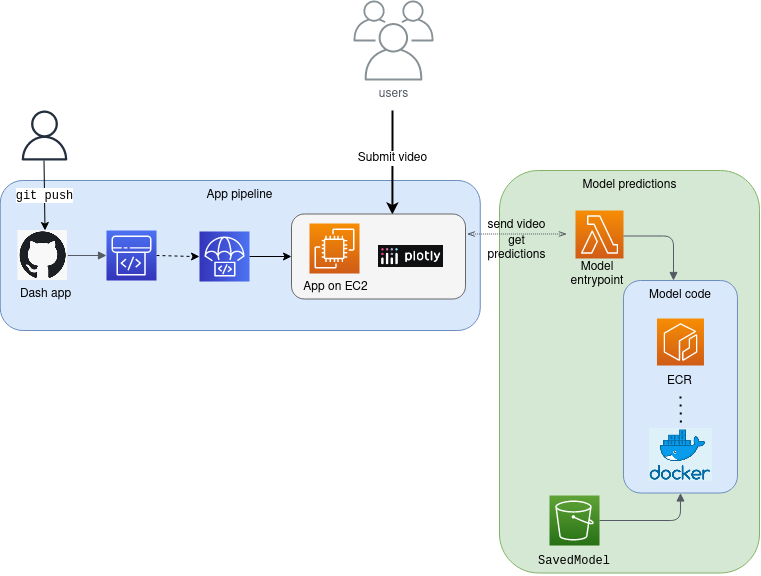
\includegraphics[width=\textwidth]{figs/cloud_diagram.png}
\caption{Diagrama Cloud}\label{cloud_diagram}


\end{figure}

\subsection{Resultado y funcionamiento}

A continuación se puede ver una serie de capturas de la app desplegada. La figura \ref{app_1} muestra la pantalla inicial de la app. La pestaña principal \textit{Clip prediction} permite cargar el vídeo arrastrando el archivo o buscándolo por su nombre. La pestaña secundaria \textit{Examples} permite ver ejemplos de los movimientos. 

\begin{figure}[H]
    \centering
		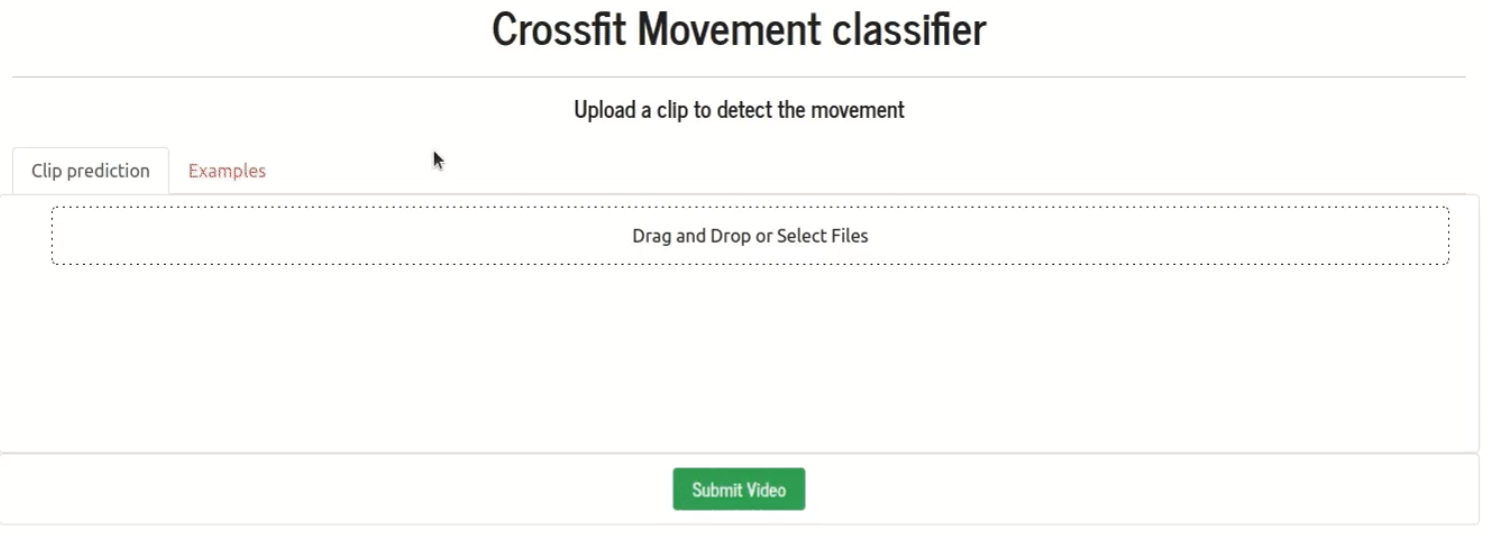
\includegraphics[width=\textwidth]{figs/app_1.png}
\caption{App: Estado inicial}\label{app_1}
\end{figure}

Una vez se ha subido un clip, este se reproduce de forma automática (figura \ref{app_2}). Para poder obtener las probabilidades asociadas al movimiento en cuestión habría que pulsar el botón \textit{Submit Video}, que envía el contenido a la función lambda.

\begin{figure}[H]
    \centering
		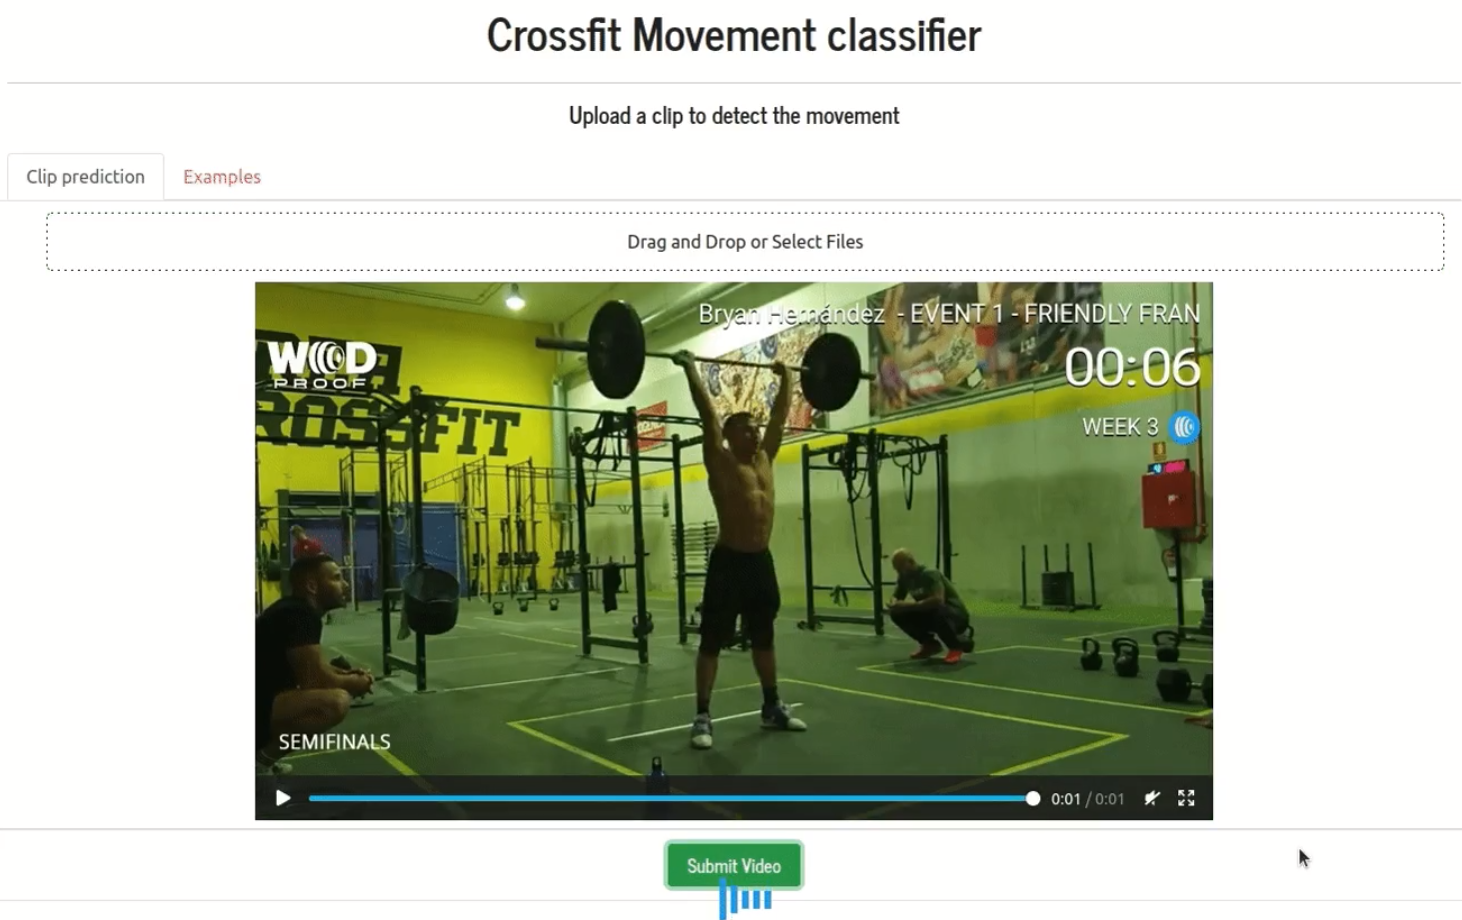
\includegraphics[width=\textwidth]{figs/app_2.png}
\caption{App: Video cargado}\label{app_2}
\end{figure}

Tras obtener la predicción del modelo, justo debajo aparece la tabla con los 5 movimientos más probables y la probabilidad asociada a cada uno de ellos, ordenados de mayor a menor, como muestra la figura \ref{app_3}.

\begin{figure}[H]
    \centering
		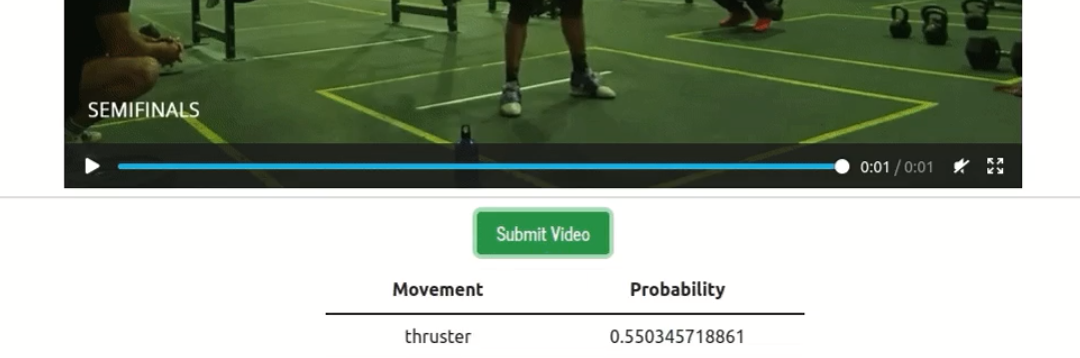
\includegraphics[width=\textwidth]{figs/app_3.png}
\caption{App: Extracto de tabla de predicciones}\label{app_3}
\end{figure}

Si bien los vídeos se han entrenado con un máximo de 10 frames, en este caso el vídeo se pasa al modelo sin hacer un muestreo de los mismos. Aunque solo se ha comprobado para unos pocos ejemplos de los vídeos completos, las probabilidades se ven afectadas, pero la ordenación de los mismos se mantiene.

El tiempo aproximado para obtener las predicciones asociadas a un clip es de alrededor de 14 segundos para un thruster, que es un movimiento relativamente corto (ver tabla \ref{table_descriptive_stats}), por lo que clasificar los movimientos es lento.

Como alternativas para ganar velocidad, se podría reducir el tamaño del modelo para mejorar la latencia de la CPU, limitando el número de posiciones decimales por ejemplo, un procedimiento conocido como \href{https://www.tensorflow.org/lite/performance/post_training_quantization}{\textit{post-training quantization}}. Los autores originales ofrecen versiones del mismo ya entrenadas para este caso \href{https://tfhub.dev/google/collections/movinet/1}{aquí}.

Existen otras alternativas. Se podría hacer un muestreo del vídeo de la misma forma que se hace durante la pipeline de entrenamiento (cabe recordar que durante el entrenamiento, el modelo solo utiliza 10 frames de cada vídeo), con lo que la información a procesar disminuiría. Otra opción sería entrenar un modelo de menor complejidad, ya sea la versión a0 o a1, ya que el accuracy actual ya es excepcionalmente alto.



 

%% Utilidades para anotaciones
\chapter{Conclusiones y trabajo futuro}\label{conclusiones}

Este trabajo presenta una aplicación de \textit{MoViNets} para la clasificación de movimientos de CrossFit, la creación de un nuevo conjunto de datos de basado en clips de videos extraídos de YouTube, con una muestra de ejercicios de CrossFit, y el desarrollo de una aplicación en AWS para la clasificación de los clips.

Como siguientes pasos se plantea el entrenamiento de las arquitecturas \textit{stream} para poder tratar videos completos en los que aparezcan distintos movimientos, y comparar este enfoque con otros como metodologías basadas en \textit{optical flow}. En cuanto al despliegue y explotación del modelo en la nube, sería interesante pasar el modelo a \textit{Tensorflow Lite} para disminuir el tamaño del mismo y mejorar los tiempos de ejecución.
 


% -------------------------------
% Apéndices
% -------------------------------
\appendix
\chapter{Anexo}

\section{Glosario de movimientos}

%\begin{minipage}{0.5\textwidth}
\begin{table}[h]
\resizebox{\textwidth}{!}{%
\centering
\label{glosario}
\begin{tabular}{lll}
\toprule
{} &                         Significado &                          Traducción \\
\midrule
thruster          &                            Thruster &                            Thruster \\
chest-to-bar      &                Chest-to-bar pull-up &                   Dominada al pecho \\
double-unders     &              Double-under rope jump &                Salto doble de comba \\
ghd               &  Glute-ham developer machine sit-up &          Abdominales en máquina GHD \\
power clean       &                         Power clean &                   Cargada de fuerza \\
deadlift          &                            Deadlift &                         Peso muerto \\
shspu             &            Strict handstand push-up &            Flexión de pino estricta \\
ohs               &                      Overhead squat &             Sentadilla de arrancada \\
bar-facing burpee &                   Bar-facing burpee &  Burpee frente a la barra con salto \\
\bottomrule
\end{tabular}
}
\end{table}
%\end{minipage}


\section{Probabilidades obtenidas por movimiento en la muestra de test}\label{Probabilidades}

En la siguiente imagen se puede ver, para cada movimiento observado, las probabilidades que devuelve el modelo.

Si nos fijamos en la imagen \textit{ohs vs rest} por ejemplo, podemos ver los movimientos entre las probabilidades que dan pie a las figuras de los heatmap de las correlaciones, figura \ref{heatmap_correlations}, donde se puede observar como cuando disminuye probabilidad de \textit{ohs}, aumenta la probabilidad de \textit{thruster}.

\begin{figure}[H]
    \centering
		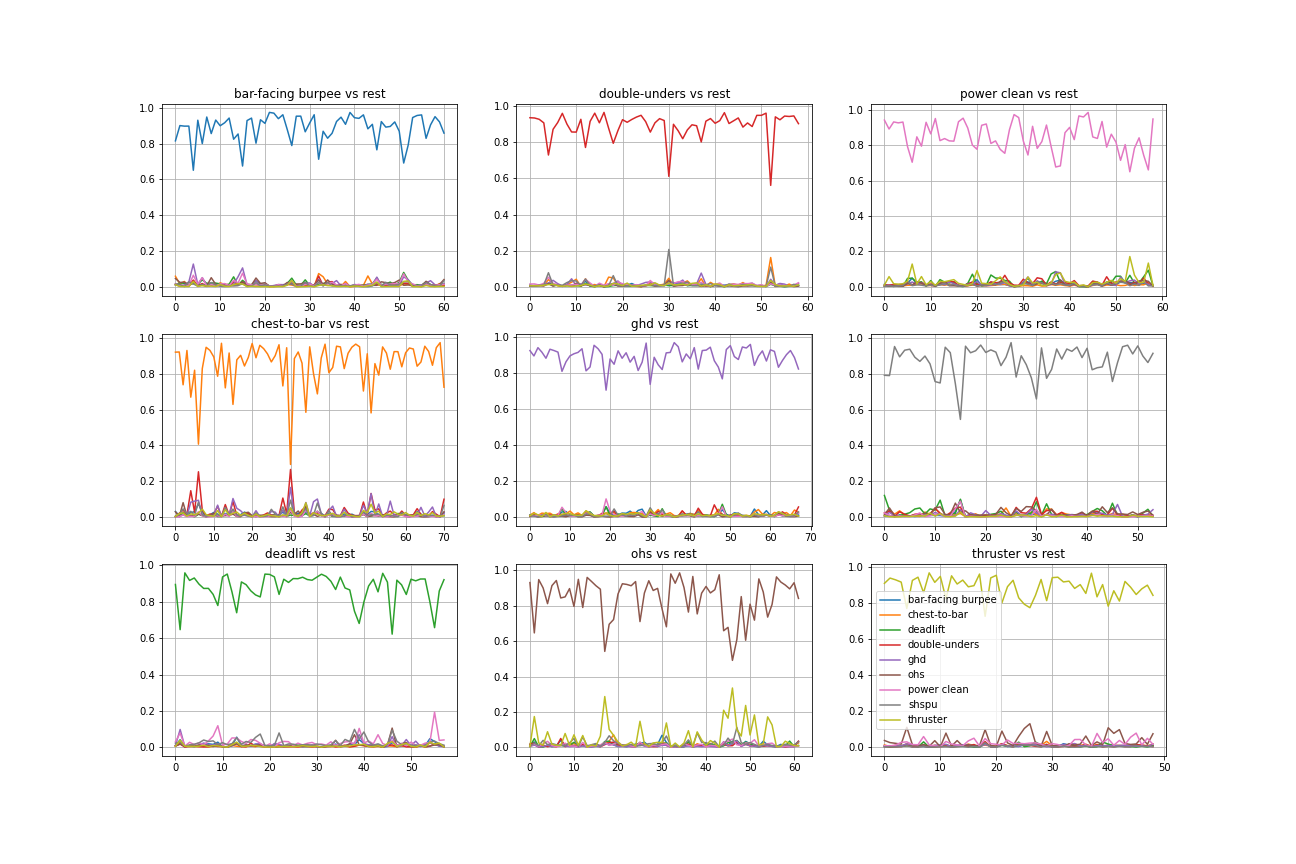
\includegraphics[width=\textwidth]{figs/probabilities_by_movement.png}
\caption{Probabilidades estimadas en la muestra de test. Para cada movimiento observado, cada gráfica representa las probabilidades obtenidas por el modelo.}\label{probabilities_by_movement}
\end{figure}



\section{Pipeline en AWS}

A la hora de tratar los videos en la función lambda hay que tener en cuenta lo siguiente, si se parte de la imagen de docker que ofrece \href{https://hub.docker.com/r/amazon/aws-lambda-python}{AWS} (como es el caso). Para leer los videos en mp4 y traducirlos a tensores para que los pueda entender tensorflow, se ha utilizado la siguiente función: \href{https://www.tensorflow.org/io/api_docs/python/tfio/experimental/ffmpeg/decode_video}{decode\_video}. Esta función parte de unos binarios que fallan en la distribución de linux que utiliza la imagen de docker, ver \href{https://github.com/tensorflow/io/issues/1648}{issue}. Como alternativa para leer los videos en este caso se ha utilizado \href{https://pypi.org/project/opencv-python-headless/}{OpenCV}, si bien el impacto impacto que tiene es mínimo a la hora de leer los clips, en los decimales usados al pasarlo a tensor.


%\chapter{Anexo 1}
%\lipsum[1-2]

%\cleardoublepage
%\clearpage
%\thispagestyle{empty}


% -------------------------------
% Bibliografía
% -------------------------------
\bibliographystyle{apalike}
\bibliography{TFM} 
\addcontentsline{toc}{chapter}{Referencia bibliográfica} % Añade a la tabla de contenidos

\end{document}